\documentclass[12pt, a4paper]{report}
\linespread{1.3}
\setlength{\parindent}{1.25cm}

\usepackage[top=3cm,left=3cm,right=2cm,bottom=2cm]{geometry}
\usepackage{indentfirst}
\usepackage{amsmath, amsthm, amsfonts, amssymb}

\usepackage{graphicx}
\usepackage{color}
\usepackage{multicol}
\usepackage[normalem]{ulem}
\usepackage{wrapfig}
\usepackage{caption}
\usepackage{fancybox}
\usepackage[pdfstartview=FitH]{hyperref}
\usepackage{subfigure}
\usepackage{acronym}
\usepackage[T1]{fontenc}		% Selecao de codigos de fonte.
\usepackage[utf8]{inputenc}
\usepackage[brazil]{babel}
\usepackage{pgfplots}   % pacote para uso do pgfplots
\usepackage{array}
\usepackage{longtable}
\usepackage{pdfpages}

\usepackage{verbatim}
\usepackage{enumitem}   
\usepackage{natbib} % criação de linhas

%Includes "References" in the table of contents
\usepackage[nottoc]{tocbibind}

\graphicspath{{Figuras/}} % caminho padrao imagens
% ------ Remove nome capitulo da tag chapter ---------
\makeatletter
\def\@makechapterhead#1{%
  \vspace*{0\p@}%
  {\parindent \z@ \raggedright \normalfont
    \interlinepenalty\@M
    \Huge\bfseries  \thechapter.\quad #1\par\nobreak
    \vskip 30\p@
  }}
\makeatother
\begin{document}

%---------- CAPA -------------

\begin{figure}[ht]
\centering

\includegraphics[scale=0.15]{UFBA.jpg}
\end{figure}

\begin{center}
\sc{\large{Universidade Federal da Bahia - UFBA}} \\
\sc{\large{Instituto de Matemática - IM}} \\
\sc{\large{Departamento de Ciência da Computação - DCC}} \\
\sc{\small{Bacharelado em Sistemas de Informação - BSI}} \\
\sc{\small{Trabalho de Conclusão de Curso}} \\

\vspace{4cm}

\sc{\Large{Sistema Colaborativo de \\Avaliação
Docente}}

\vspace{4.5cm}

\sc{\Large{Kênia Arruda Guimarães}}

\vspace{5.5cm}

\textbf{Salvador - Bahia} \\
Dezembro de 2019

\end{center}
\thispagestyle{empty}

%---------- FOLHA DE ROSTO -------------
\newpage
\begin{center}
\sc{\Large{Sistema Colaborativo de \\Avaliação
Docente}}

\vspace{4cm}

\large{Kênia Arruda Guimarães}
\end{center}

\vspace{4cm}

\begin{flushright}
\begin{minipage}{8.6cm}
Monografia apresentada como trabalho de conclusão de curso para o curso de Bacharelado em Sistemas de Informação do Departamento de Ciência da Computação na Universidade Federal da Bahia.

\vspace{0.5cm}
\textbf{Orientador}: Prof. Dr. Rodrigo Rocha Gomes e Souza.

\end{minipage}
\end{flushright}
 
\vspace{7cm}

\begin{center}
\textbf{Salvador - Bahia} \\
Dezembro de 2019
\end{center}



%%%%%%%%%%%%%%%%%%%%%%
% Ficha Catalográfica
\newpage
\thispagestyle{empty}
\null\vfill
                  
\begin{center}
 Ficha catalográfica.
\begin{tabular}{|p{13.5cm}|}%{p{12cm}}
\hline
\begin{small}
\begin{verbatim}
Guimarães, Kênia Arruda
Sistema Colaborativo de Avaliação Docente - UFBA. / Kênia
Arruda Guimarães. - Salvador, 01, 2019.
60.:il.
Orientador: Rodrigo Rocha Gomes e Souza.
Monografia (Graduação) - UNIVERSIDADE FEDERAL DA BAHIA,
INSTITUTO DE MATEMÁTICA, 07 de dezembro de 2019.
TÓPICOS PARA FICHA CATALOGRÁFICA.
I.  Souza, Rodrigo Rocha Gomes e. 
II. UNIVERSIDADE FEDERAL DA BAHIA. INSTITUTO DE MATEMÁTICA.
III Título.
                                                  NUMERO CDD
\end{verbatim}
\end{small}
\\ \hline
\end{tabular}
\end{center}
%\setcounter{page}{2} %truque para não numerar a página


%---------- BANCA EXAMINADORA -------------
\newpage
\begin{center}
\sc{\Large{\textbf{Termo De Aprovação}}}
\vspace{1.3 cm}
\par\sc{\Large{Sistema Colaborativo de \\Avaliação Docente}}

\vspace{2cm}

\large{Kênia Arruda Guimarães}
\end{center}

\vspace{1.3 cm}

\begin{flushright}
\begin{minipage}{8.6cm} 
Monografia apresentada como trabalho de conclusão de curso para o curso de Bacharelado em Sistemas de Informação do Departamento de Ciência da Computação na Universidade Federal da Bahia.
\end{minipage}
\end{flushright}
 
\vspace{1cm}
\begin{center}
\Large \textbf{Banca Examinadora:}
\end{center}
\vspace{1cm}

\begin{flushright}
\begin{minipage}[l]{12cm}
\begin{center}
\uline{\hspace{10.5cm}} \\
Prof. Dr. Rodrigo Rocha Gomes e Souza (Orientador) \\ Universidade Federal da Bahia \\
\vspace{1cm}
\uline{\hspace{10.5cm}} \\
Prof. Dra. Débora Abdalla Santos \\ Universidade Federal da Bahia \\
\vspace{1cm}
\uline{\hspace{10.5cm}} \\
Prof. Fulano de Tal \\ Universidade Federal da Bahia \\


\end{center}
\end{minipage}
\end{flushright}

%-----------Dedicatória----------------
\newpage
\vspace*{21cm}
\begin{flushright}
\textit{Dedico este trabalho à minha família}
\end{flushright}


%------------Agradecimentos------------
\newpage
\chapter*{Agradecimentos}
\thispagestyle{empty}
\par Aos meus pais que sempre estiveram ao meu lado me apoiando em cada decisão tomada.

À minha noiva Juliana Alves Pereira que vem sendo meu maior suporte incentivo neste ciclo de aprendizado. 

Aos meus amigos e em especial à Lina Mendes que me deu grande auxílio no design da aplicação e ao Carlos Henrique e Ludmila Cruz que sempre tiveram muita paciência ao ouvir os desabafos quando ainda não tinha encontrado a solução para alguns dos obstáculos que encontrei durante a a execução deste projeto. 

Ao meu orientador Rodrigo Rocha Gomes e Souza pela excelente orientação, paciência e atenção prestados no desenvolvimento deste trabalho e a Universidade Federal da Bahia (UFBA) pelo espaço público de ensino que mesmo com todas as dificuldades encontradas forma excelentes profissionais que vem contribuindo constantemente para o desenvolvimento do nosso país.  

%------------Citação-------------------
\newpage
\vspace*{20cm}
\begin{flushright}
\begin{minipage}{8cm}
\begin{flushright}
\textit{
"Toda a ciência é nada mais do que um refinamento do pensamento cotidiano". \\
Albert Einstein}
\end{flushright}
\end{minipage}
\end{flushright}


%--------------Resumo-------------------
\newpage
\chapter*{Resumo}
\thispagestyle{empty}


%-------------Abstract------------------
\newpage
\chapter*{Abstract}
\thispagestyle{empty}

%-------------Índice--------------------
\newpage
\tableofcontents
\thispagestyle{empty}

% ----------- Lista de figuras ----------

\pdfbookmark[0]{\listfigurename}{lof}
\listoffigures
\cleardoublepage

%--------- Lista de tabelas ---------

\pdfbookmark[0]{\listtablename}{lot}
\listoftables
\cleardoublepage

%--------- Lista de Siglas---------
\chapter*{Lista de Siglas}
\addcontentsline{toc}{chapter}{Lista de Siglas} 

\begin{acronym}
\acro{SICAD}{Sistema Colaborativo de Avaliação Docente}
\acro{SIAC}{Sistema de Avaliação Docente}
\acro{UFBA}{Universidade Federal da Bahia}
\acro{SUPAC}{Superintendência de Administração Acadêmica}
\acro{IES}{Instituições de Ensino Superior}
\acro{SIGAA} {Sistema Integrado de Gestão de Atividades} 
\end{acronym}


%-------------Capítulo 1-----------------
\chapter{Introdução}
\section{Contexto}
\section{Problema}
\section{Solução}

%-------------Capítulo 2-----------------

\chapter {Trabalhos Relacionados}


\section{RateMyProfessors}
O RateMyProfessors \footnote{RateMyProfessors. Disponível em <\url{www.ratemyprofessors.com}>. Acesso em: 17 nov. 2019.} é um site de avaliação institucional, onde foi concebido em maio de 1999 por John Swapceinski. Inicialmente o site foi lançado como TeacherRatings e depois para RateMyProfessors no ano de 2001. O sistema permite que os discente de universidades atribuam classificações a docentes de instituições americanas, canadenses e do Reino Unido.

A plataforma é tem como foco a avaliação de professores utilizando conceitos como nível de dificuldade, atribuições de palavra de tags(palavras chaves) como por exemplo "respeitoso", "faz muitos artigos", "atividades para casa" e etc. É possível cadastrar professores caso eles não estejam na base de dados e os comentários e avaliações são anônimos.

Para ser publicado, o usuário deve classificar o curso e/ou professor em uma escala de barra de 1 a 5 nas seguintes categorias: "qualidade geral" e "nível de dificuldade". O avaliador também pode compartilhar se eles levariam o professor novamente, se a aula foi tirada para crédito, se a participação é obrigatória, se o livro didático é usado, qual nota eles receberam no curso e incluir comentários de até 350 caracteres no máximo. comprimento. Os avaliadores também podem selecionar até 3 tags que descrevem o professor em uma lista de 20. Na figura \ref{fig:ratemyprofessor} visualizamos a inserção de uma avaliação docente.

\begin{figure}
\centering
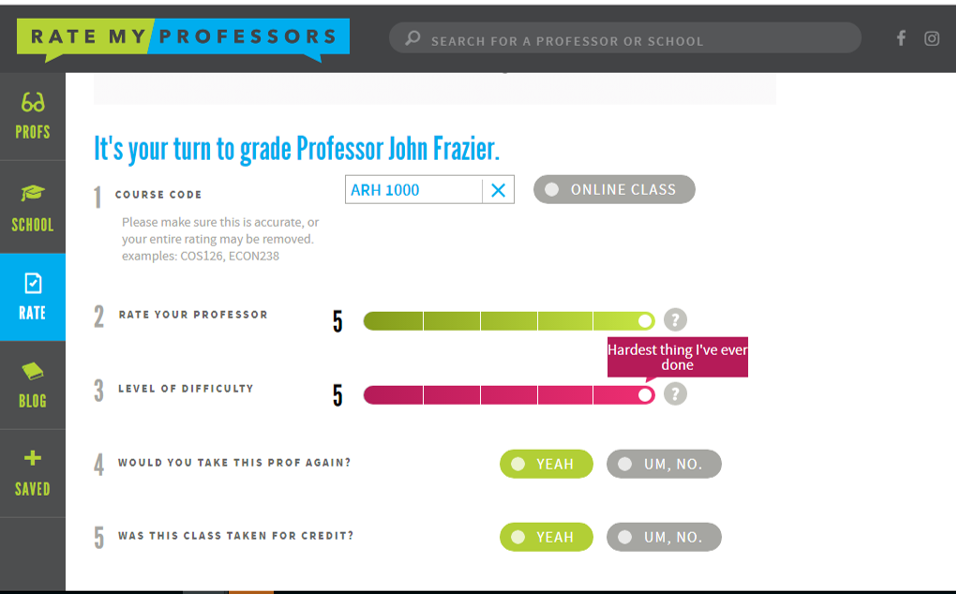
\includegraphics[scale=0.45]{ratemyprofessor.png}
\caption{Processo de Avaliação Docente do site RateMyProfessors.}
\label{fig:ratemyprofessor}
\end{figure}

\section{RateMyTeachers}

O RateMyTeachers\footnote{RateMyTeachers. Disponível em <\url{www.ratemyteachers.com/}>. Acesso em: 17 nov. 2019.} assim como RateMyProfessor é um site de avaliação institucional porém seu publico alvo é a classificação de professores de ensino fundamental e médio e escolas. Os usuários podem classificar seus professores em uma escala de 1 a 5 nas categorias facilidade, utilidade, conhecimento e clareza, com os dois últimos considerando uma pontuação de "qualidade geral". É permitido realizar comentários sobre as experiências com os professores.

O site foi lançado em 2001 pela Mister Message e posteriormente vendido ao ex-proprietário Patrick Nagle Atualmente o site atende instituições de ensino nos Estados Unidos, Reino Unido, Canadá, Irlanda, Austrália e Nova Zelândia .

Um fato pertinente referente ao RateMyTeachers é que inicialmente o mesmo era moderado por uma comunidade pública de voluntários. Esta comunidade pública foi substituída em 2017 por uma comunidade privada de moderação que se encarrega de revisar manualmente todas as classificações e professores adicionados ao site desde 2001. Podemos observar na figura \ref{fig:ratemyteacher} o processo inicial de inserção de uma avaliação docente.

\begin{figure}
\centering
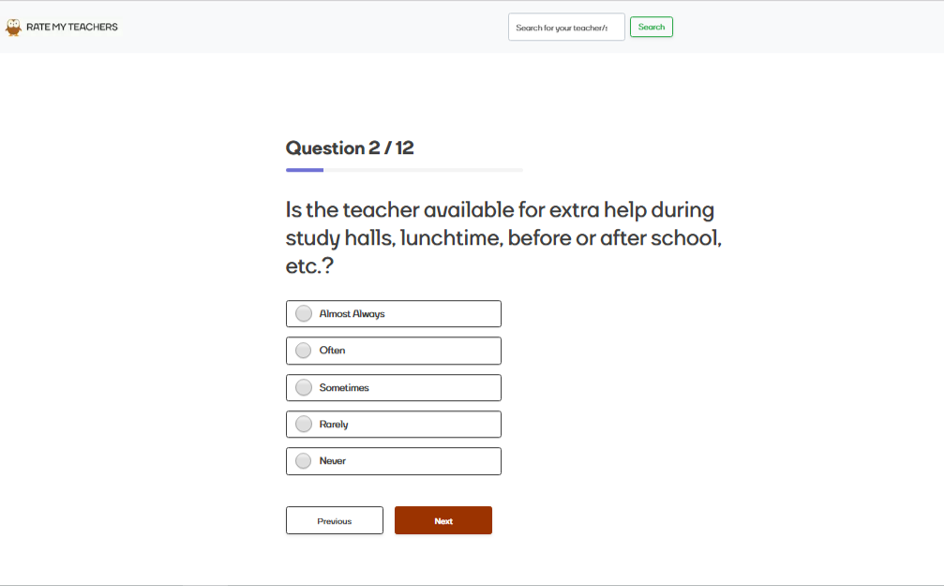
\includegraphics[scale=0.45]{ratemyteachers.png}
\caption{Processo de Avaliação Docente do site RateMyTeachers.}
\label{fig:ratemyteacher}
\end{figure}

\section{Avaliação Docente Instituições de Ensino Superior}

 A Lei Federal nº 10.861, de 14 de abril de 2004, instituiu o Sistema Nacional de Avaliação da Educação Superior (SINAES), que prevê que toda instituição de ensino superior(IES), pública ou privada, constituirá uma Comissão Própria de Avaliação (CPA), responsável pela autoavaliação da instituição.  O SINAES avalia todos os aspectos que giram em torno de alguns eixos principais. São eles o ensino,a responsabilidade social, a pesquisa, a extensão, a gestão da instituição,o desempenho dos alunos, as instalações e o corpo docente.
 
 Toda instituição deverá realizar o levantamento de informações referente a avaliação institucional. No que tange a UFBA essas informações são coletas através de sistemas de informações como o Sistema de Avaliação Docente, o SIAV para os cursos de graduação e o Sistema Integrado de Gestão de Atividades Acadêmicas, SIGAA para os cursos de pós graduação onde é envolvendo a comunidade acadêmica (docentes e discentes).
 
 %Cada instituição forma sua CPA
 



%-------------Capítulo 3-----------------
\chapter{Solução Proposta: SICAD}

Como solução para a problemática apresentada neste trabalho, está sendo proposto o Sistema Colaborativo de Avaliação Docente, SICAD, como ferramenta auxiliar para os discentes da Universidade Federal da Bahia utilizarem, a fim de disponibilizar feedbacks e avaliações sobre as disciplinas cursadas. 

O processo de concepção do SICAD foi realizado inicialmente como uma junção do trabalho já realizado pelo Sistema de Avaliação Docente, o SIAV\footnote{SIAV. Disponível em <\url{www.siav.ufba.br/siav/privado/index.faces}>. Acesso em: 11 nov. 2019.} disponibilizado pela \ac{UFBA}.\footnote{UFBA. Disponível em <\url{www.ufba.br}> . Acesso em: 1 nov. 2019.} com uma funcionalidade de se realizar comentários, que será especificada no subtópico a seguir. A partir deste escopo foram traçados os requisitos da solução que serão descritos abaixo.

\section{ Modelo Conceitual}
Por definição \textbf{modelo conceitual} é um conjunto de suposições baseadas no mundo real que indicarão as regas de negócio de um sistema \citep{mapaconceitual}.

A importância do desenvolvimento de um mapa conceitual no contexto deste trabalho é a representação gráfica do modelo proposto, referente os processos relacionados ao \ac{SICAD}, a fim de que ele possa ser entendido de forma fluída.

Existem três macros processos   

\section{ Autenticação}

Inicialmente foi pensado em um login básico para autenticação no sistema, possuindo apenas usuário e senha. Entende-se como login o processo para acessar um sistema informático restrito, utilizando credenciais que são previamente cadastradas pelo usuário nesse sistema com a finalidade da identificação do utilizador. Contudo, analisando o contexto da aplicação o login abrangeria qualquer usuário logado na internet que possuísse o caminho do sistema, não sendo interessante, pois os mesmos teriam acesso a resultados que possuem informações sensíveis.

Para delimitar o acesso ao \ac{SICAD}, foi utilizado o módulo de \href{https://www.autenticacao.ufba.br}{autenticação} disponibilizado pela \ac{UFBA}. Seu emprego segue o seguinte processo: a aplicação no ato do login, faz uma requisição à autenticação da \ac{UFBA} e a mesma retorna o username \footnote{Username. Disponível em <\url{www.cartilha.cert.br/senhas/}> . Acesso em: 1 nov. 2019.} caso o usuário possua cadastro na universidade. Na figura \ref{fig:processo_autenticacao} é demonstrado o fluxograma do processo.

\begin{figure}
\centering
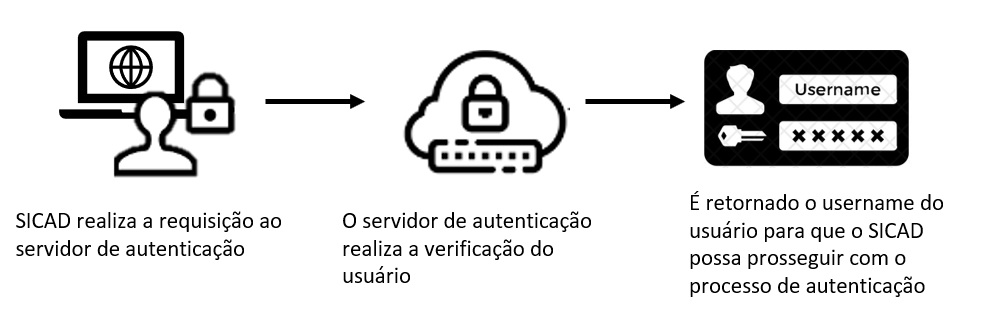
\includegraphics[scale=0.50]{processo_autenticacao.jpg}
\caption{Fluxograma da Requisição de Autenticação}
\label{fig:processo_autenticacao}
\end{figure}

Dessa forma o acesso ao \ac{SICAD} é restrito a quem possui cadastro na universidade, não expondo assim informações indevidas à usuários que não são elegíveis para utilizar o sistema.

\subsection{Usuário e Segurança}

No processo de desenvolvimento da autenticação ficou claro a necessidade da implementação de uma camada de segurança, visto que a resposta à requisição feita juntamente a \ac{UFBA} retorna o username do usuário sem nenhum tipo proteção.
A segurança da informação é essencial no sentido de preservar o valor dessa informação que é chave para a maioria das funcionalidades do \ac{SICAD}. Focando neste ponto foram implementadas rotinas para prover segurança nos processos executados pelo sistema que serão descritos nos passos abaixo:

\begin{itemize}
\item o usuário tenta logar no sistema, consequentemente disparando uma requisição para a autenticação da \ac{UFBA};
\item A \ac{UFBA} executa todas as rotinas de validação.
Caso se obtenha uma resposta positiva, retorna o username do usuário sem proteção para a aplicação que solicitou a requisição;
\item O \ac{SICAD} antes de persistir a informação no banco de dados, utiliza da tecnologia de criptografia Hash SHA256\footnote{Hash SHA256. Disponível em <\url{www.tsapps.nist.gov/publication/get_pdf.cfm?pub_id=910977}> . Acesso em: 2 nov. 2019.}, que será abordada no tópico 3.6. para criptografar o username utilizado como informação chave na utilização do sistema. 
\end{itemize}

Para melhor fixação, o fluxo do processo está representado na figura \ref{fig:fluxograma_criptografia}. 

\begin{figure}
\centering
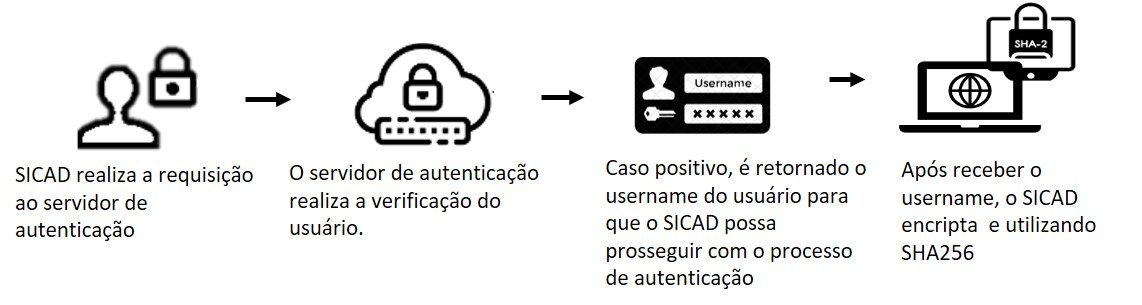
\includegraphics[scale=0.80]{fluxograma_criptografia.jpg}
\caption{Fluxograma das Etapas do Processo de Criptografia do Username.}
\label{fig:fluxograma_criptografia}
\end{figure}

Por conseguinte, com o usuário criptografado e devidamente protegido, a integridade da informação será mantida sendo assim confiável que o usuário utilize o sistema de forma segura.

\section{ Perfis}
A utilização de perfis de usuários está atrelada a restrição de acesso à certas funcionalidades do sistema, que embora não elimine todos os riscos à segurança da informação mas diminui incidentes que possam ocorrer, comprometendo ao conjunto de critérios de segurança conhecido como o tripé da segurança da informação: \textbf{confidencialidade}, \textbf{integridade} e \textbf{disponibilidade}:

\begin{itemize}
\item \textbf{Confidencialidade:} É a garantia de que a informação é acessível somente por pessoas autorizadas a terem acesso \cite{iso27002};
\item \textbf{Integridade:} É a garantia da exatidão e completeza da informação e dos métodos de processamento \cite{iso27002};
\item \textbf{Disponibilidade:} É a garantia de que os usuários autorizados obtenham acesso à informação e aos ativos correspondentes sempre  que necessário. \cite{iso27002}
\end{itemize}

No \ac{SICAD} foi implementado controle de perfis considerando critérios de segurança acima para que não ocorra a quebra dos mesmos gerando venerabilidades.

\subsection{O controle de Acesso}

Um processo de segurança essencial assegurado pelos critérios de segurança é o controle de acessos. É difícil imaginar como qualquer sistema teria condições minímas de continuar funcionando sem ele e por isso é imprescindível sua implementação.

\subsection{Controle  de  Acesso  Baseado  em  Papéis }

Considerando o cenário dos acessos que foram pensados para o \ac{SICAD}, foi escolhido o modelo de \textbf{controle  de  acesso  baseado  em  papéis} devido a sua adequação à aplicação.

Para \citep{sandhu1997} o modelo Role Based Access Control – RBAC flexibiliza o gerenciamento do controle de acesso através da adição de um componente que intermedeia usuários e permissões. Este, considera quatro componentes básicos:
\begin{itemize}
\item \textbf{Usuários}: Podem ser seres humanos ou outros agentes autônomos,tais como robôs,agentes de softwares e computadores;
\item \textbf{Permissões}: São os direitos de executar uma ou mais ações ou operações sobre objetos do sistema;
\item \textbf{Papéis}: São os intermediários entre os usuários e as permissões. Em vez de conceder permissões diretamente aos usuários, as permissões são concedidas aos papéis. Papéis são funções distintas dentro do sistema, como por exemplo Administrador, Moderador e etc. Usuários são associados a um ou mais papéis.  
\item \textbf{Sessões}: Quando um usuário acessa o sistema, ele inicia uma \textbf{sessão}, durante  essa  sessão, pode haver  um  ou  mais  papéis ativos. Conforme a especificação do modelo, o usuário pode ter ou não o poder de decidir quais papéis ativar em um dado momento.
\end{itemize}

Partindo desses quatro componentes foram criados os papéis e permissões do sistema que poderão ser visualizados através da tabela abaixo:

% ######## init table ########
\begin{table}[h]
 \centering
% distancia entre a linha e o texto
 {\renewcommand\arraystretch{1.25}
 \begin{tabular}{ l l }
  \cline{1-1}\cline{2-2}  
    \multicolumn{1}{|p{3.850cm}|}{\textbf{Papel} \centering } &
    \multicolumn{1}{p{4.217cm}|}{\textbf{Permissão} \centering }
  \\  
  \cline{1-1}\cline{2-2}  
    \multicolumn{1}{|p{3.850cm}|}{Administrador} &
    \multicolumn{1}{p{4.217cm}|}{incluir, alterar, visualizar, bloquear, desbloquear em todos os módulos do sistema.}
  \\  
  \cline{1-1}\cline{2-2}  
    \multicolumn{1}{|p{3.850cm}|}{Utilizador} &
    \multicolumn{1}{p{4.217cm}|}{incluir, alterar, ocultar e mostrar nos módulos de comentários e avaliação.}
  \\  
  \hline
 \end{tabular} }
 \caption{Papéis e Permissões}
\end{table}

Um usuário poderá ter o papel de administrador ou utilizador associado. Como padrão quando o mesmo realiza o login já é atribuído à ele o papel de \textbf{utilizador}.
\par Além dos papéis e permissões citados acima, o \ac{SICAD} conta com módulos, que são partes do sistema responsáveis por uma tarefa definida, que estão por sua vez associados aos papéis como é demonstrado pela tabela abaixo:
% ######## init table ########
\begin{table}[h]
 \centering
% distancia entre a linha e o texto
 {\renewcommand\arraystretch{1.25}
 
 \begin{tabular}{ l l }
  \cline{1-1}\cline{2-2}  
    \multicolumn{1}{|p{3.850cm}|}{\textbf{Módulo} \centering } &
    \multicolumn{1}{p{7.217cm}|}{\textbf{Papel} \centering }
  \\  
  \cline{1-1}\cline{2-2}  
    \multicolumn{1}{|p{3.850cm}|}{Comentário} &
    \multicolumn{1}{p{6.217cm}|}{Administrador, Utilizador}
  \\  
  \cline{1-1}\cline{2-2}  
    \multicolumn{1}{|p{3.850cm}|}{Avaliação} &
    \multicolumn{1}{p{6.217cm}|}{Administrador, Utilizador}
  \\  
    \cline{1-1}\cline{2-2}  
    \multicolumn{1}{|p{3.850cm}|}{Resultados} &
    \multicolumn{1}{p{6.217cm}|}{Administrador, Utilizador}
  \\  
    \cline{1-1}\cline{2-2}  
    \multicolumn{1}{|p{3.850cm}|}{Ajuda} &
    \multicolumn{1}{p{6.217cm}|}{Administrador, Utilizador}
  \\  
    \cline{1-1}\cline{2-2}  
    \multicolumn{1}{|p{3.850cm}|}{Carga} &
    \multicolumn{1}{p{6.217cm}|}{Administrador}
  \\  
    \cline{1-1}\cline{2-2}  
    \multicolumn{1}{|p{3.850cm}|}{Moderação} &
    \multicolumn{1}{p{6.217cm}|}{Administrador}
  \\  
    \cline{1-1}\cline{2-2}  
    \multicolumn{1}{|p{3.850cm}|}{Configurações} &
    \multicolumn{1}{p{6.217cm}|}{Administrador}
  \\  
  \hline
 \end{tabular} }
 \caption{Papéis e Módulos}
\end{table}
%rever https://www.teses.usp.br/teses/disponiveis/3/3141/tde-08032013-120904/publico/TeseEduardoTakeoUeda.pdf%

O modelo RBAC além de impedir que um usuário possua papéis conflitantes com ele é possível impor restrições aos papéis, resultando em mais proteção e boa gestão da informação oferecida pelo sistema.
\section{ Principais Funcionalidades}

O \ac{SICAD} foi pensado como uma junção da funcionalidade de avaliar os docentes da universidade tal como é realizado semestralmente através do \ac{SIAC} com uma nova funcionalidade de realizar comentários.

Os \textbf{comentários} são uma forma do discente compartilhar sua experiência vivida na sala de aula e que poderá ser visualizada por todos os usuários que são elegíveis para utilizar o sistema.

As \textbf{avaliações} são um parecer que um discente fornece referente a um docente e seu trabalho ministrando uma dada disciplina, em um dado semestre. O conceito de avaliação foi baseado no que já utilizado pela universidade.

Contabilizando as avaliações realizadas pelos estudantes é oferecido pelo \ac{SICAD} os \textbf{resultados}, onde são apresentadas de forma simples e transparente a contabilização dos itens avaliados.

O utilizador do sistema possui também do recurso de \textbf{ajuda} onde poderá tirar dúvida a respeito do que são comentários, avaliações e resultados em qualquer momento. Podemos observar na figura \ref{fig:home_administrador} a tela incial do sistema.
\begin{figure}
\centering
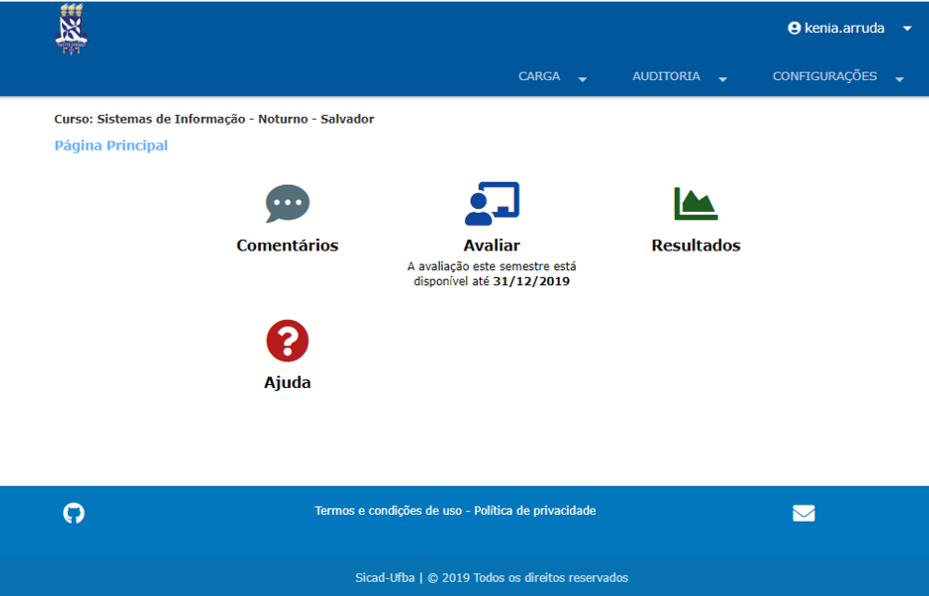
\includegraphics[scale=0.5]{home_administrador.png}
\caption{Tela Inicial do SICAD.}
\label{fig:home_administrador}
\end{figure}

Nos próximos tópicos serão descritos as principais funcionalidades de cada módulo disponível no \ac{SICAD}.

\subsection{Comentário}
Um comentário tem por objetivo o compartilhamento das experiências vividas e informações pertinentes de uma determinada combinação de disciplina+professor+semestre cursada. Espera-se que sejam compartilhadas informações que gerem conhecimento base para os que não conhecem a disciplina e/ou o trabalho do professor naquela disciplina.

Além dos objetivos citados, os comentários também poderão ser utilizados como sugestões, elogios e críticas sobre o conhecimento ministrado na disciplina+professor+semestre avaliada.

Os comentários no \ac{SICAD} deverão seguir a convenção de não possuir palavras de baixo de calão, gerando assim constrangimento. Abaixo um exemplo de comentário:

\begin{table}[h]
 \centering
 {\renewcommand\arraystretch{1.25}
 \begin{tabular}{ l l }
  \cline{1-1}\cline{2-2}  
    \multicolumn{1}{|p{7.850cm}|}{\par \textbf{Disciplina:} Álgebra Linear
    \par \textbf{Professor:} Fulano de Tal
    \par \textbf{Comentário:} Esse professor é muito atencioso! Aprendi a disciplina rapidamente. Acho que ele passa muito trabalho extra classe.}
  \\  
  \hline
 \end{tabular}}
 \caption{Exemplo de Comentário}
\end{table}

O módulo de comentário possui as seguintes ações:

\begin{itemize}
\item \textbf{Incluir}: Esta funcionalidade permite o usuário incluir um comentário que ficará disponível para os demais usuários. Uma vez realizado, o mesmo passa a possuir a situação de \textbf{comentário público}. Fica obrigatório o utilizador informar a disciplina, o semestre, o professor e o comentário a ser realizado. Na figura \ref{fig:incluir_comentario} observamos um exemplo a tela de inclusão.

\begin{figure}
\centering
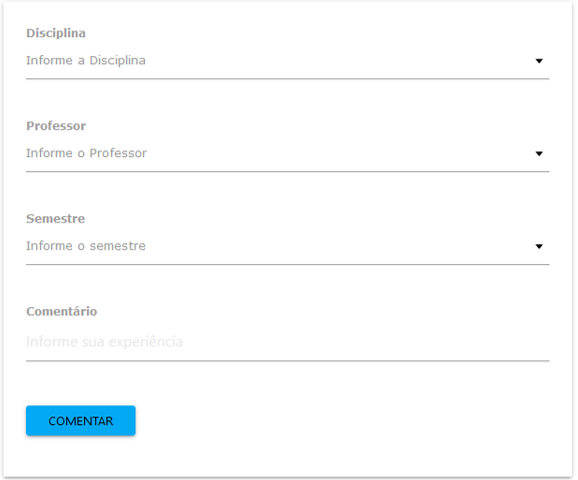
\includegraphics[scale=0.6]{incluir_comentario.png}
\caption{Tela de Inclusão de Comentário.}
\label{fig:incluir_comentario}
\end{figure}

\item \textbf{Visualizar}: Esta funcionalidade permite ao usuário consultar tanto os seus próprios comentários realizados como os que foram incluídos por outros usuários. Podemos visualizar nas figuras \ref{fig:comentarios} e\ref{fig:visualizacao_meu_comentario} respectivamente; 

\begin{figure}
\centering
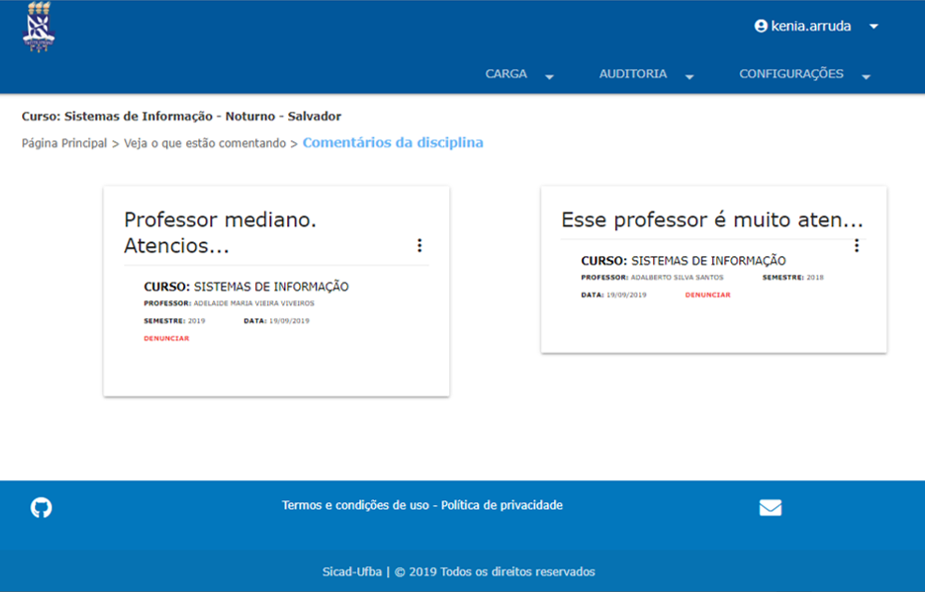
\includegraphics[scale=0.5]{comentarios.png}
\caption{Tela de Visualização de Todos os Comentários.}
\label{fig:comentarios}
\end{figure}

\begin{figure}
\centering
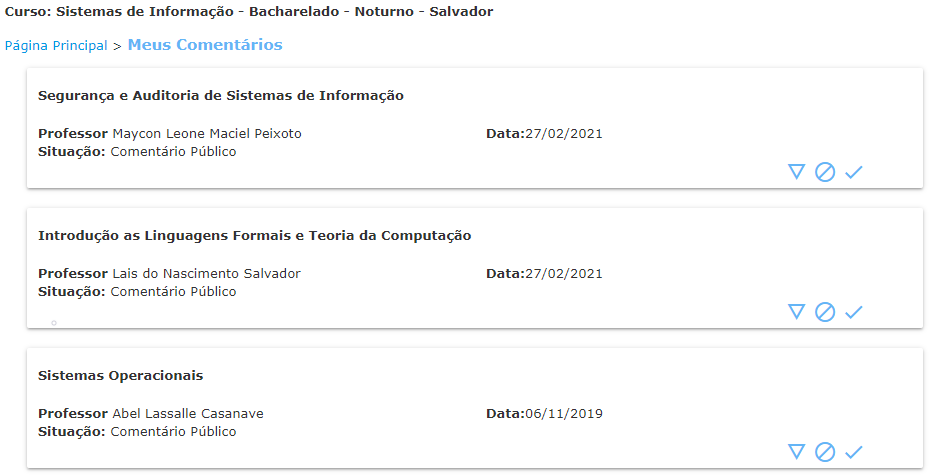
\includegraphics[scale=0.5]{visualizacao_meu_comentario.png}
\caption{Tela de Visualização dos Comentários Realizados pelo Usuário.}
\label{fig:visualizacao_meu_comentario}
\end{figure}

\item \textbf{Ocultar/Mostrar}: Estas funcionalidades respectivamente permitem ao usuário ocultar um comentário realizado, ou seja, esse comentário não poderá ser mais visualizado pelos demais, passando a ter a situação de \textbf{comentário oculto}, podendo apenas ser consultado pelo próprio utilizador e para revogar o privilegio de ocultamento o mesmo poderá utilizar a função de mostrar, tornando o \textbf{comentário publico} novamente. Nas figuras \ref{fig:comentario_oculto} e \ref{fig:comentario_publico} visualizamos os exemplos.

\item \textbf{Denunciar}: Um comentário poderá ser denunciado quando o mesmo infringir a convenção, ou seja, ter palavras de baixo calão em seu conteúdo. Comentários escritos de forma pejorativa dissonante dos objetivos propostos deverão ser denunciados. Todos os participantes que utilizam \acro{SICAD} poderão denunciar comentários inapropriados.
\begin{figure}
\centering
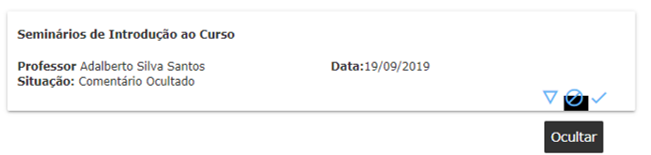
\includegraphics[scale=0.7]{comentario_oculto.png}
\caption{Imagem de um Comentários Oculto.}
\label{fig:comentario_oculto}
\end{figure}

\begin{figure}
\centering
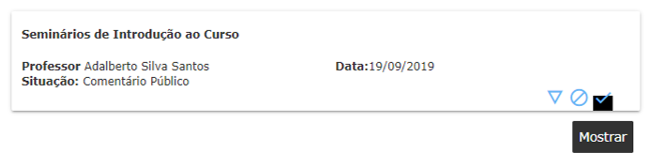
\includegraphics[scale=0.7]{comentario_publico.png}
\caption{Imagem de um Comentários Público.}
\label{fig:comentario_publico}
\end{figure}

\end{itemize}
\subsection{Avaliação}

Uma avaliação é uma análise que um discente fornece referente a um docente e/ou seu trabalho ministrando uma dada disciplina, em um dado semestre. Ela é composta de avaliações sobre a didática, relacionamento com os alunos e domínio de conteúdo, uma escala de recomendação e atribuições de palavras-chaves(tags). A avaliação é uma combinação professor+disciplina+semestre que são itens geralmente levados em consideração para uma decisão da matricula de um aluno.

O módulo de avaliação possui as seguintes ações:
\begin{itemize}
\item \textbf{Incluir}: Esta funcionalidade permite o usuário incluir uma avaliação docente onde serão avaliados os critérios de didática, relacionamento com os alunos e domínio de conteúdo, baseados nos mesmos conceitos utilizados pelo SIAV onde será atribuído um gostei ou não gostei à cada item.

O usuário pode associar palavras-chaves (tags) na inclusão da avaliação. Ao final o mesmo deverá informar na escala de 1 a 5 estrelas qual o nível de recomendação do docente lecionando a disciplina avaliada. Por padrão a recomendação está apontada para o 3. 

Fica obrigatório o utilizador informar a disciplina, o semestre, o professor. Na Figura \ref{fig:incluir_avaliacao}  podemos visualizar a tela de inclusão de uma avaliação docente.

\begin{figure}
\centering
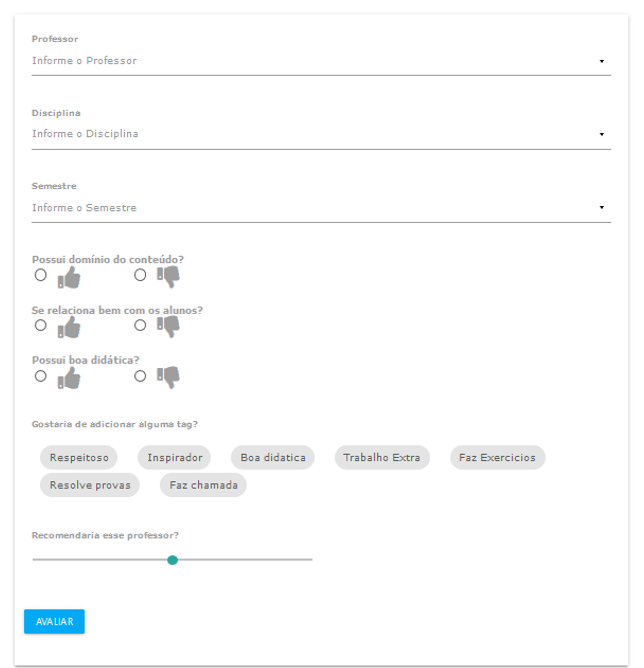
\includegraphics[scale=0.47]{incluir_avaliacao.png}
\caption{Incluindo uma Avaliação Docente.}
\label{fig:incluir_avaliacao}
\end{figure}

\item \textbf{Visualização}: Esta funcionalidade permite o usuário visualizar suas avaliações realizadas. Na figura \ref{fig:visualizacao_minha_avaliacao} observamos as avaliações do utilizador.

\begin{figure}
\centering
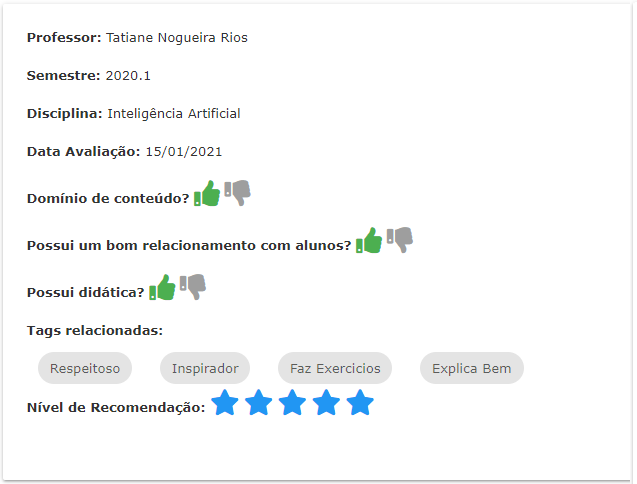
\includegraphics[scale=0.5]{visualizacao_minha_avaliacao.png}
\caption{Visualização das Avaliações do Usuário.}
\label{fig:visualizacao_minha_avaliacao}
\end{figure}

\end{itemize}
\subsection{Resultados}
Um resultado tem como objetivo demonstrar de forma sintética as avaliações realizadas ao longo do semestre, auxiliando assim o discente na escolha das disciplinas que irão compor sua  grade.

Os resultados são apresentados por semestre e dentro do mesmo serão visualizados os resumos por professor. Na figura \ref{fig:resultados} observamos um exemplo de resultado.

\begin{figure}
\centering
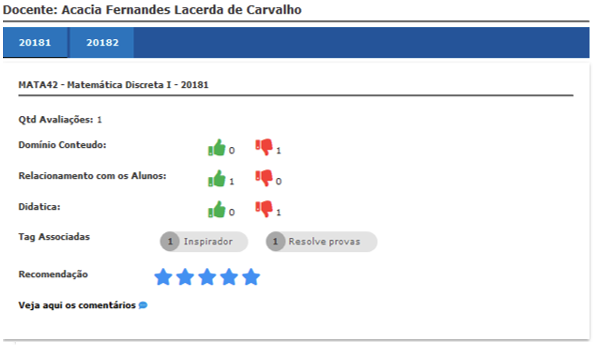
\includegraphics[scale=0.7]{resultados.png}
\caption{Demostração dos Resultados.}
\label{fig:resultados}
\end{figure}

Como é visualizado na imagem \ref{fig:resultados}, uma contagem do conceito de "gostei" e "não gostei" dos itens domínio de conteúdo, relacionamento com o aluno e didática é apurada. É realizada também a contagem da quantidade que uma palavra-chave foi associada na avaliação. Já para a recomendação, na sua contabilização é utilizada a média ponderada dada pela formulação matemática :

\begin{equation}
\frac{\sum_{n}^{i-1}(pi*xi)}{\sum_{n}^{i-1}(pi)} 
\end{equation}

Através dos resultados os discente poderão visualizar os comentários de acordo com a disciplina, o semestre e o professor selecionado.

\subsection{Ajuda}

Pensando na experiência do utilizador e para proporcionar uma ferramenta de respostas à questionamentos frequentes foi disponibilizado um módulo de ajuda para os usuários do SICAD.
Nele é possível tirar dúvidas acerca do que são comentários, avaliação e resultados. Podemos visualizar na figura \ref{fig:ajuda} o módulo de ajuda.

\begin{figure}
\centering
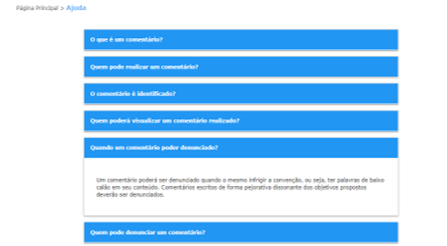
\includegraphics[scale=0.9]{ajuda.png}
\caption{Demonstração da Ajuda.}
\label{fig:ajuda}
\end{figure}

\subsection{Carga}
As informações sobre os cursos, disciplinas e professores que são utilizados no sistema, são disponibilizadas para o público no site da Superintendência de Administração Acadêmica\footnote{SUPAC. Disponível em <\url{www.supac.ufba.br}>. Acesso em: 13 nov. 2019} (SUPAC) na forma de um documento HTML.

Na captura dos dados citados acima foi utilizado um processo conhecido como  \textit{web scraper}. Para \cite{laender2002} um web scraper é uma sequência de procedimentos que são realizados afim de ser obter informações de páginas na web usando bots, conhecidos como scrapers. Essas informações posteriormente podem ser usadas para análise de dados.

Segundo \cite{Glezscraping2013} um \textit{web scraping} ou raspagem de dado pode ser definido como o processo de extração e combinação de conteúdo de
interesse da Web de maneira sistemática.

Para \cite[p. 1]{ilprints376} em tradução livre um crawler "coleta automaticamente páginas da Web para criar um índice local e / ou local coleção de páginas da web.", ou seja, é um programa que coleta informação em paginas da internet, podendo criar índices e/ou armazenar esses dados bem como atualizá-los. 

O processo de desenvolvimento do web scraping foi baseado no trabalho realizado por \citeauthor{assis2017meuhorario} no projeto do MeuHorário2\footnote{MeuHorário2. Disponível em <\url{www.meuhorarioufba.com.br/}>. Acesso em: 13 nov. 2019}. Inicialmente foram definidas tês etapas, utilizando o tipo informação que passa a ser o foco da extração: cursos, disciplinas e professores.  Em cada etapa, foi desenvolvida uma task conceito utilizado pela linguaguem de programação ruby \footnote{Ruby. Disponível em <\url{www.docs.ruby-lang.org/en/2.2.0/Rake/Task.html}>. Acesso em: 13 nov. 2019.}, que são tarefas, ou seja, instruções a serem executadas mesmo que a aplicação não esteja em execução. 

A primeira tarefa desenvolvida foi a extração de cursos de uma página de listagem dos cursos da UFBA. Foram extraídos os dados: nome e código do curso. Podemos visualizar na figura \ref{fig:lista_cursos}.

\begin{figure}
\centering
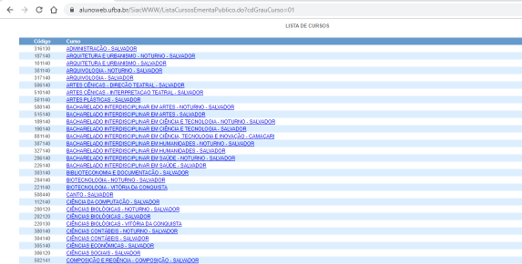
\includegraphics[scale=0.9]{lista_cursos.png}
\caption{Lista de Cursos.}
\label{fig:lista_cursos}
\end{figure}

A segunda tarefa desenvolvida foi a extração das disciplinas de cada curso. No site da \acro{SUPAC} existe uma área que possui links para os guias de matrícula de cada curso. Os cursos são divididos por áreas e a partir dos guias, é possível obter informações sobre as disciplinas sendo assim habilitada uma associação entre curso x disciplina. Na figura \ref{fig:disciplinas} podemos visualizar um exemplo da demonstração das disciplinas de um curso.

\begin{figure}[ht!]
\centering
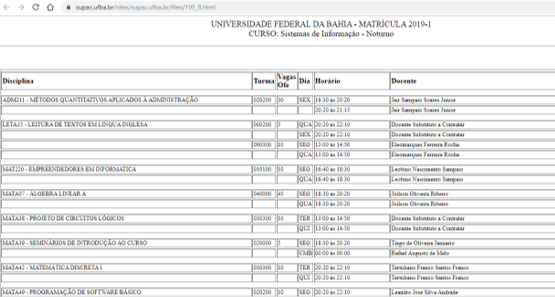
\includegraphics[scale=0.8]{disciplinas.png}
\caption{Lista de Disciplinas de um Curso.}
\label{fig:disciplinas}
\end{figure}

Finalizando o conjunto das tarefas, a extração da relação dos professores também se dá pelo guia de matricula visto que a partir dele é possível obter a informação dos professores como é representado na figura \ref{fig:disciplinas} . 

\subsection{Moderação}
Para \citep{netosolanca2007}, a auditoria é uma atividade que reúne a análise das operações, processos, sistemas e responsabilidades gerenciais de uma determinada entidade, com o intuito de validar sua conformidade com certos objetivos e políticas institucionais, regras, orçamentos, normas ou padrões.
Partindo do conceito de auditoria, uma das suas vertentes seria a moderação de conteúdo. Este por sua vez se encaixa no contexto do SICAD, pois os comentários realizados embora deverão seguir do padrão de não possuir palavras de baixo calão, os palavrões, podem se tornar ofensivos havendo a necessidade de uma intervenção do moderador.
De acordo com \cite{SMITH2019} existem quatro tipos de moderação:
\begin{itemize}
\item \textbf {Pré-moderação: }Com a pré-moderação, você emprega moderadores para verificar novamente o conteúdo enviado pelo seu público-alvo antes que ele fique visível ao público; 
\item \textbf {Pós-moderação: }Ao contrário da pré-moderação, a pós-moderação abre caminho para conversas em tempo real e postagem imediata, porque o conteúdo é verificado depois de publicado. ;
\item \textbf {Moderação distribuída: }Um sistema de classificação é usado com moderação distribuída, permitindo que os membros da comunidade votem em determinados envios. Um exemplo de moderação distribuída é o stackoverflow onde os usuários votam nas respostas mais adequadas para uma pergunta realizada;
\item \textbf {Moderação automatizada: }A moderação automatizada funciona usando aplicativos específicos de moderação de conteúdo para filtrar certas palavras ofensivas e conteúdo multimídia. A detecção de postagens inapropriadas se torna automática e mais integrada. 
\end{itemize}

O SICAD utiliza dois dos tipos de moderações citados que são os de pós moderação e moderação automatizada. Devido ao seu conteúdo sensível os comentários são moderados quando necessário. Como dado pessoal sensível a lei Nº 13.709, de 14 de agosto de 2018 artigo 5º nos diz "Dado pessoal sensível é informação relativa a origem racial ou étnica, convicção religiosa, opinião política, filiação a sindicato ou organização, saúde, vida sexual ou dado genético ou biométrico.".  Contudo, o artigo 5º nos fornece um conceito de dado sensível muito engessado e entendo que a informação armazenada referente aos comentários que são registrados no sistema pode de algum jeito gerar constrangimento se exposta, foi desenvolvido um modulo de moderação dos comentários realizados pelos usuários.

A moderação neste momento inicial será realizada por um usuário com papel Moderador associado a ele. Observa-se a pós moderação, quando o moderador pode visualizar todos os comentários realizado, e os que forem denunciados ou tiver seu conteúdo escrito de forma pejorativa, poderão de bloqueá-los. Quando bloqueado, o comentário automaticamente não ficará mais disponível para consulta dos demais. Também é papel do Moderador manter atualizada a lista de palavras restritivas utilizada pela rotina de inserção de comentários. 


A moderação automatizada foi implementada pensando em não permitir que o usuário realize um comentário pejorativo auxiliando o moderador e mantendo um feed saudável com elogios e criticas construtivas. Utilizando a técnica stemmização, que segundo \cite{porter1980} em tradução livre “stemmer” é um processo para remover as palavras morfológicas e nas terminações flexionais mais comuns das palavras. Seu principal uso é como parte de um processo de normalização de termo que geralmente é feito ao configurar sistemas de Recuperação de Informação”, quando o usuário escreve um comentário e nele possui alguma palavra que está contida numa lista de palavras restritivas previamente preenchida o comentário não é persistido no banco de dados.  

Através dos pontos citado acima podemos entender a importância da utilização da moderação dentro das organizações e sistema pois é  mais uma camada que auxilia na segurança da informação no critério de integridade contribuindo para a sua consistência.

\subsection{Configuração}
O módulo de configuração foi implementado para que se pudesse realizar as configurações básicas para que o SICAD possa funcionar de acordo com a estrutura proposta. Nele o Administrador pode dar cadastrar e dar manutenção nas palavras chaves utilizadas pela avaliação, nas palavras restritivas utilizadas no módulo de comentários e informar o período em que a avaliação ficará disponível para utilização dos usuários.

\section{ Anonimato}

Considerando a definição de anonimato pertencente ao Dicionário UNESP do português contemporâneo " 1- ausência de notoriedade; 2-obscuridade; 3- que ou que é obscuro, desconhecido: que ou o que não tem nome ou renome." \cite[p. 75]{da2004dicionario} 


\section{ Segurança}



%-------------Capítulo 4-----------------
\chapter{Avaliação}
\par descrever um pouco do processo de avaliação
\section{Objetivo da avaliação }
\par  Colocar aqui o porquê dos formulário e beta tester
\section{Forma de avaliação }
\par descrever como onde e quando foi aplicado o formulario
\section{Resultados } 
\par apresentar os gráficos;
%-------------Capítulo 5-----------------
\chapter{Considerações Finais}

%-------------Bibliografia------------------

\renewcommand\bibname{Referências}
\bibliographystyle{apa}
%\bibliographystyle{abntex2-alf}
%\bibliographystyle{unsrt}
\bibliography{referencias}
\nocite{*}


%-------------Apêndice------------------
\appendix
\chapter{Apêndice}

\label{whatever}


\end{document}
